\documentclass[12pt]{article}
\usepackage{listings}
\usepackage{inputenc}
\usepackage{graphicx}
\usepackage{float}
\usepackage{array}

\lstset{
	extendedchars=\true,
	language=Matlab,
	basicstyle=\tiny;
	columns=fullflexible,
	numbers=left,
	frame=single,
	breaklines=true,
	postbreak=\mbox{{$\hookrightarrow$}\space},
}
\renewcommand{\thesubsubsection}{\alph{subsubsection} )}




\begin{document}

\title{Addon zu den Übungsaufgaben I, SBV1 }
\author{Lisa Panholzer, Lukas Fiel}
\maketitle


\newpage
\section{Übungsaufgaben I, addon}
\subsection{Stressanalyse}

\subsubsection{Recherche}

\subsubsection{Analyse der EKG Sequenzen}

\subsubsection{Herzratenvariablität}

\subparagraph{Analyse des Hautleitwerts}

\newpage
\subsection{Geschwindigkeitsermittlung}
\label{sec:Geschwindigkeitsermittlung}
\subsubsection{Ermittlung von Geschwindigkeit und Distanz}
\textit Aufgabenstellung:
Zu untersuchen war ein Datensatz, der mit Daten eines Beschleunigungssensors gefüllt war. Bekannt war, dass es sich um die Daten einer geradlinigen Bewegung entlang einer Tischkante handelte die etwa 2 m lang war. Neben den Daten des Sensors waren auch Zeitstempel enthalten. In Figure \ref{fig:plainData} ist gut zu erkennen, dass die Werte des Datensatzes bereits bearbeitet wurden. Diese Tatsache wurde in der Vorlesung erwähnt. Unseres Wissens wurde eine Baseline - Korrektur durchgeführt und alle Werte der Messung bis zur zu beobachtenden Bewegung wurden 0 gesetzt. 

\textit Idee:

Eine ersten Auswertung der Daten mittels Octave zeigt Figure \ref{fig:plainData}. Ein reines Aufsummieren der Werte vermittelte einen ersten Eindruck.
Die Summe der Messungen (im Folgenden "Geschwindigkeit" genannt) ist an diesem Punkt aber negativ. Da wir von einer Ruhelage des Objekts am Ende der Bewegung ausgehen gilt es diesen Wert zu korrigieren. 

\begin{figure}[H]
	\centering
	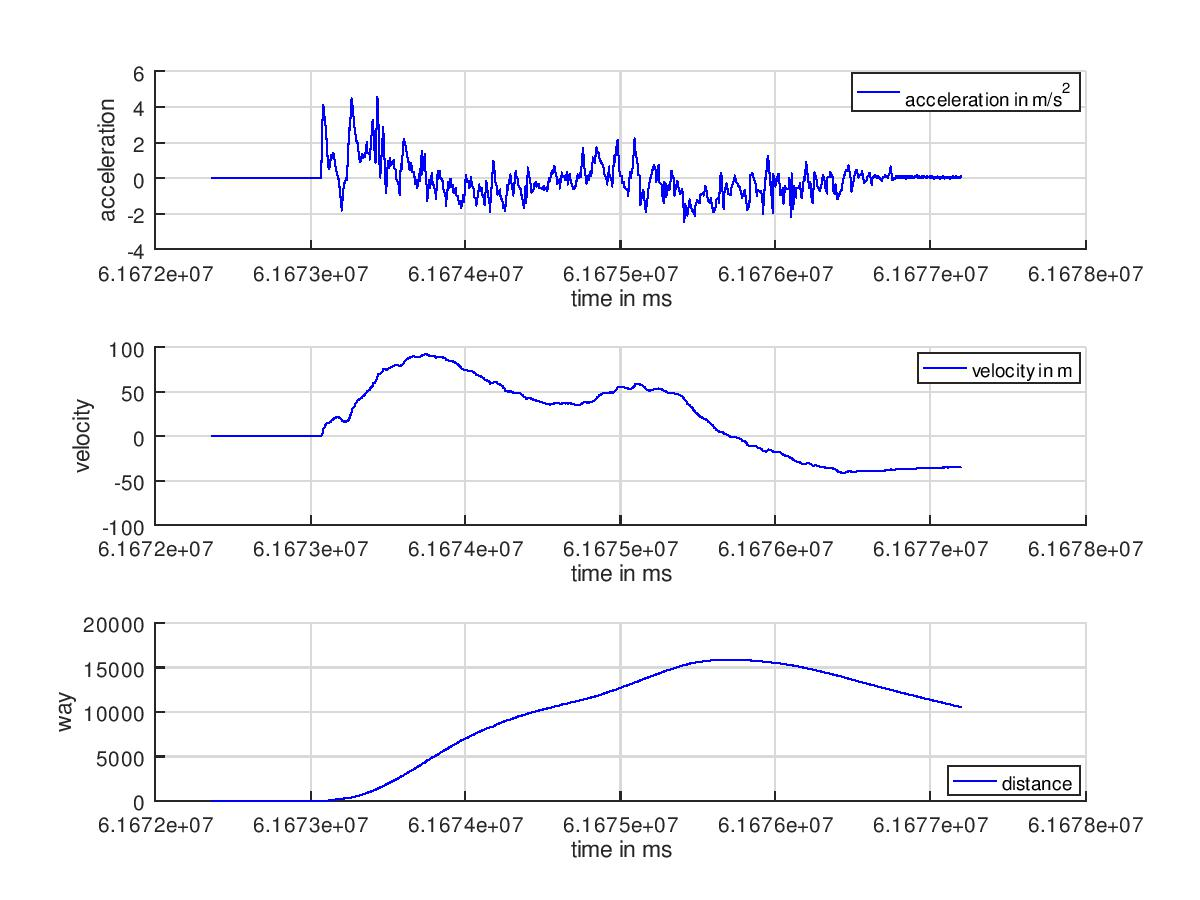
\includegraphics[width=10cm]{images/testData.jpg}
	\caption{Die Daten des Beschleunigungssensors wurden aufsummiert um die Geschwindigkeit zu erhalten. Dieser Prozess wurde wiederholt um einen ersten Eindruck über ein mögliches Wegsignal zu gewinnen.}
	\label{fig:plainData}
\end{figure}

\textit Korrektur:

Die Beschleunigungsdaten werden mittels eines gleitenden Mittelwerts gefiltert. Jeder Wert unter einem gewissen Threshold wird zu 0 gesetzt. Weil am Ende der Messung nur leichtes Rauschen erkennbar ist, können diese Werte zu 0 gesetzt werden was ein Erkennen des Bereichs der interessanten Bewegung möglich macht. 
Nach dem Aufsummieren der Beschleunigungsdaten muss sich nun darum gekümmert werden, dass die Geschwindigkeit am Anfang und Ende der Messung 0 ist. Da die anfänglichen Daten sowieso 0 sind muss nur das Ende betrachtet werden. Hier erkennt man eine wesentliche Abweichung. Es wird ein linearer Fehler angenommen, den es zu korrigieren gilt, wesshalb eine linear ansteigende Korrektor des Offset implementiert wurde. 
Aus den so gewonnenen Geschwindigkeitsdaten konnte wiederum der zurückgelegte Weg durch Summation berechnet werden.
Eine Abbildung der bearbeiteten Daten zeigt Figure \ref{fig:filteredData}. Die Auswertung ergibt, dass der mittels bearbeiteten Daten errechnete Weg ( $ 15866$mm ) viel weiter als der durch die gefilterten Daten errechnete Weg ( $21412.68931$mm ) von der Annahme einer Bewegung über $2$ m Distanz abweicht.

\begin{figure}[H]
	\centering
	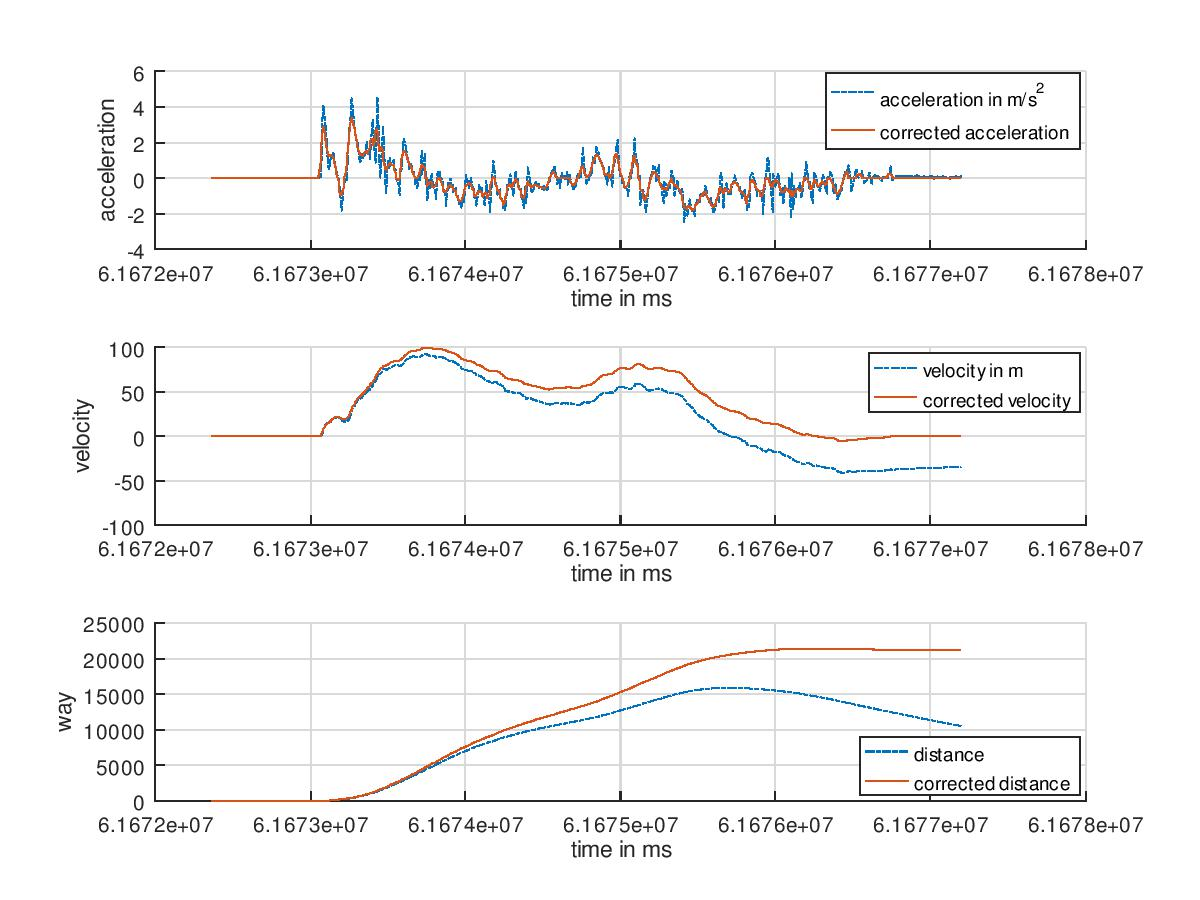
\includegraphics[width=10cm]{images/filteredData.jpg}
	\caption{Gefilterte und korrigierte Darstellung der Daten.}
	\label{fig:filteredData}
\end{figure}


\newpage
\lstinputlisting[frame=single,breaklines=true]{../accelerometerProcessing.m}

\end{document}
